\begingroup
\let\figure\RSIappendixfigure
\let\endfigure\RSIendappendixfigure
\subsubsection{Original four-round Qwen figures}
\label{app:qwen-raw-figures}

Figures~\ref{fig:qwen-raw-unaudited}--\ref{fig:qwen-raw-comparison-difficulty}
show the original Qwen3-1.7B plots for rounds 0--4.
The unaudited and audited runs are shown separately and together,
including their difficulty-stratified curves. The plotted observations
are the same as those summarized in Figure~\ref{fig:qwen-four-round}
and Tables~\ref{tab:qwen-endpoints} and~\ref{tab:qwen-rounds}; these
plots are not additional experiments. Each uses the same 2,000 ID
or 1,000 OOD questions across checkpoints and five paired blocks.
Error bars are pointwise, descriptive 95\% block-$t$ intervals;
round zero is one shared base checkpoint, not five independent fits.
The underlying observations and intervals are unchanged.

\begin{figure}[H]
\centering
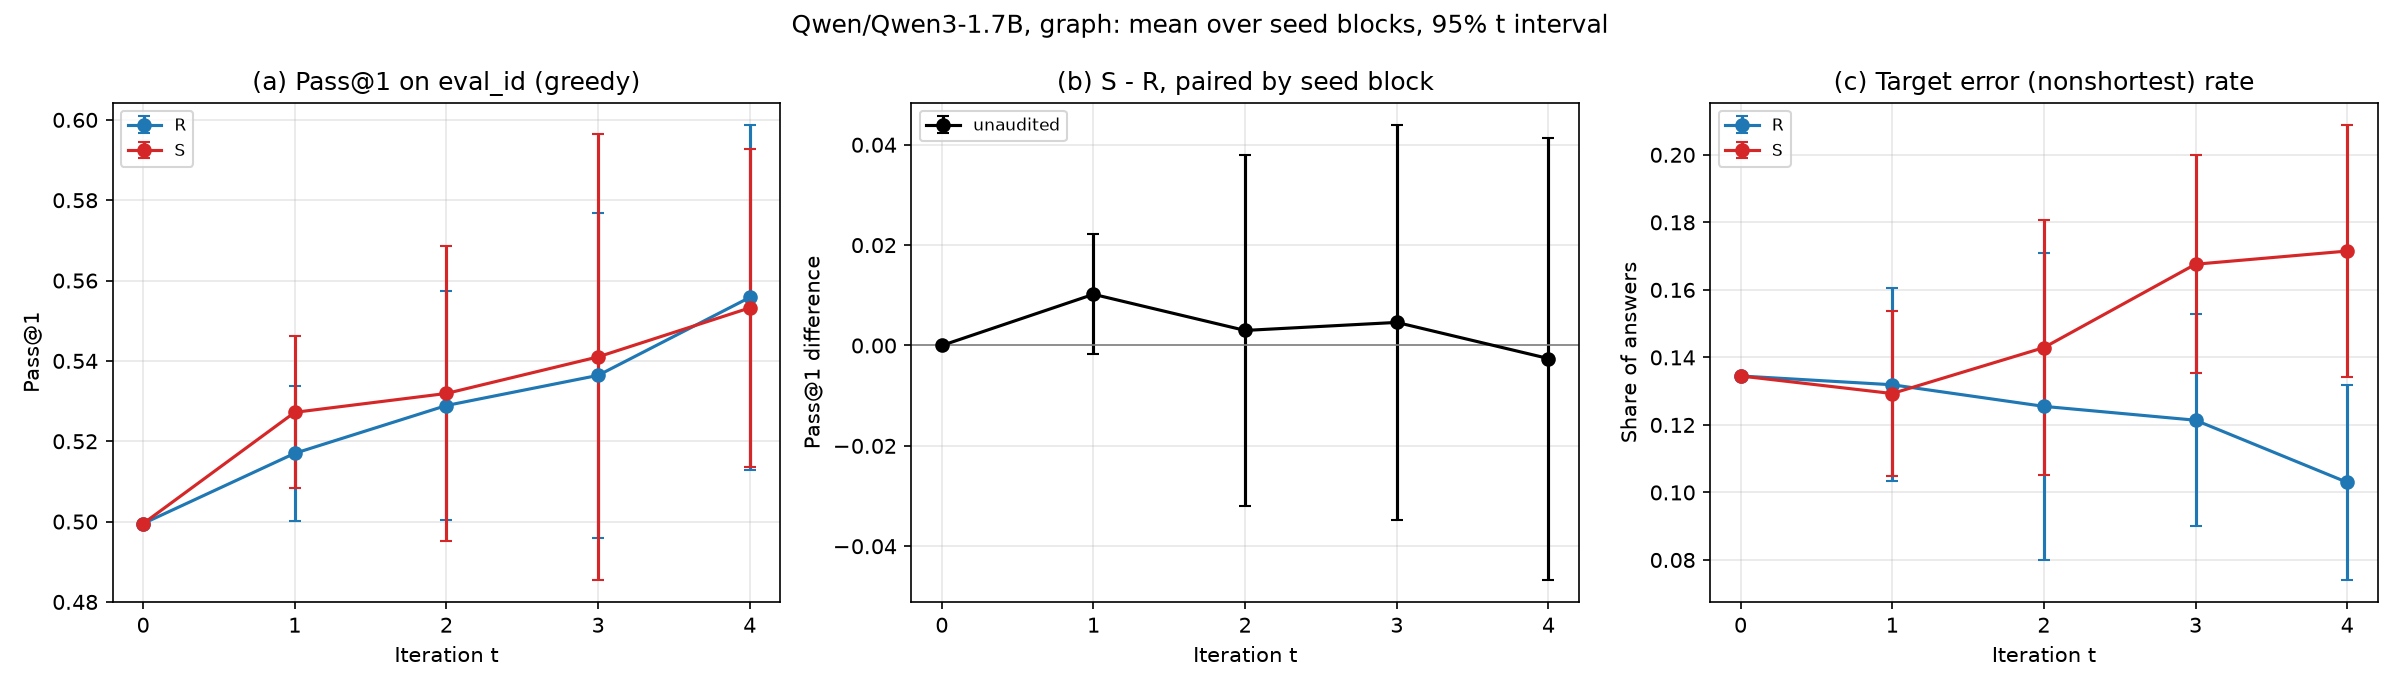
\includegraphics[width=0.90\linewidth]{figures/qwen_four_round_raw/unaudited_eval_id_pass1.png}
\par\smallskip
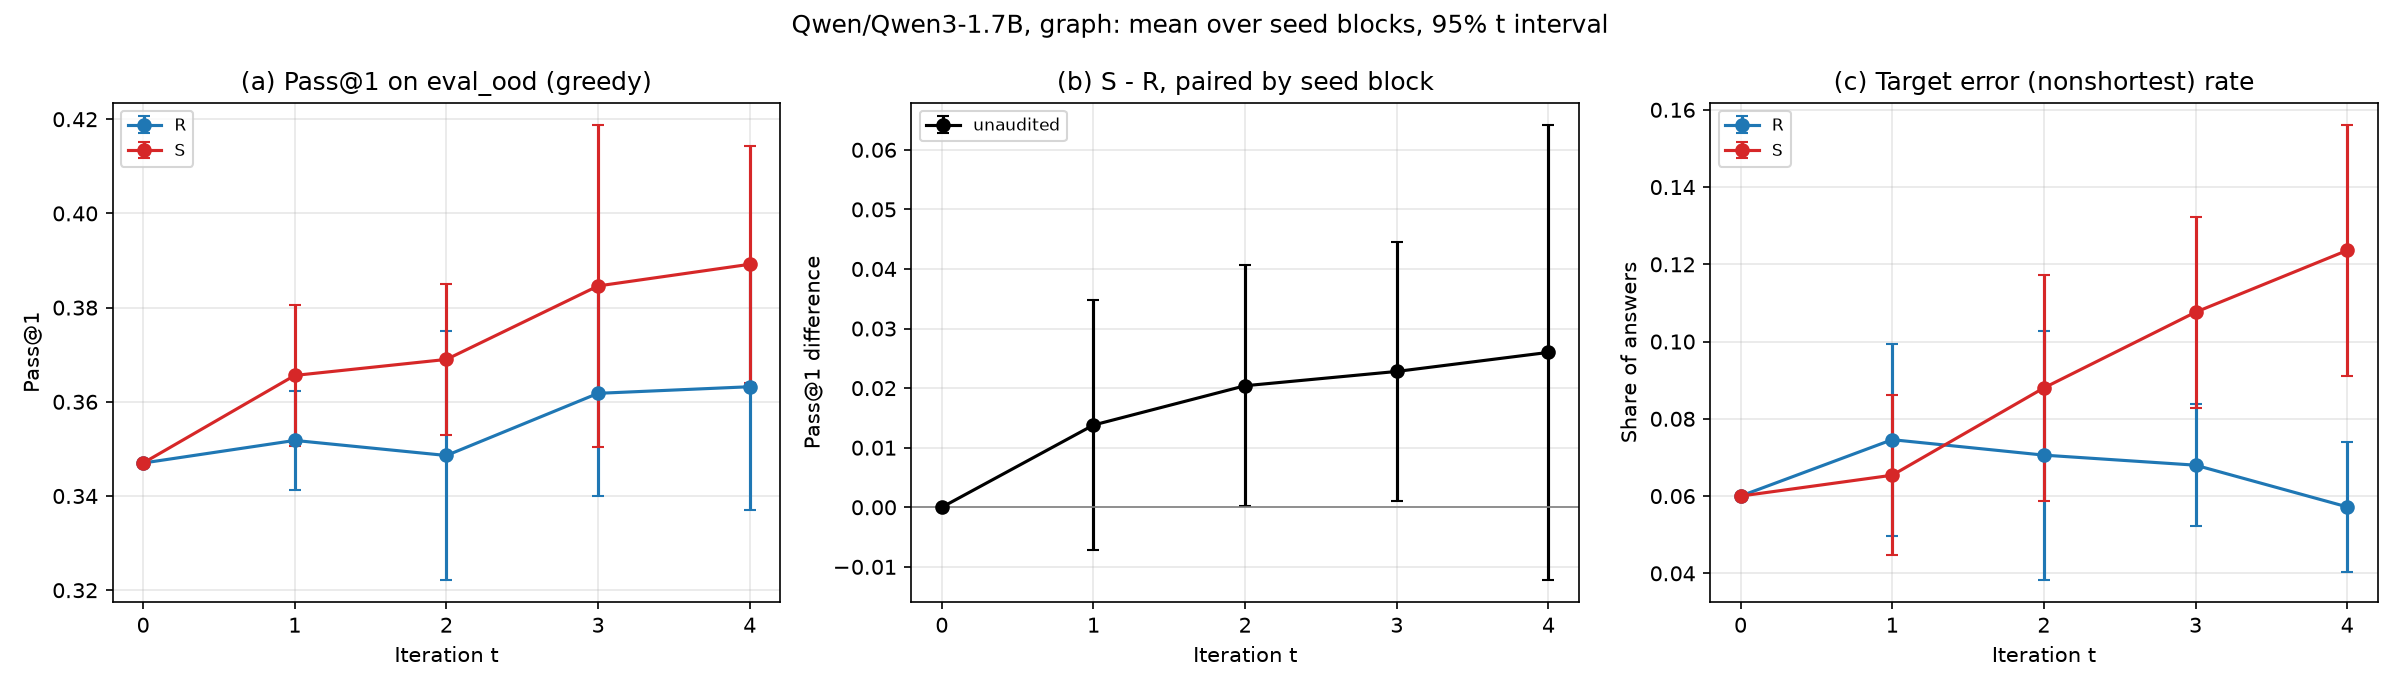
\includegraphics[width=0.90\linewidth]{figures/qwen_four_round_raw/unaudited_eval_ood_pass1.png}
\caption{Original unaudited Qwen3-1.7B graph curves, ID (top) and OOD
(bottom), for rounds 0--4. The three panels show greedy Pass@1, paired
$S-R$ accuracy, and nonshortest-error incidence among all answers.}
\label{fig:qwen-raw-unaudited}
\end{figure}

The unaudited arms reach round-four accuracy $0.556/0.553$ ID and
$0.363/0.389$ OOD, up from the common bases $0.4995$ and $0.3470$.
Nonshortest-error contrasts are $0.068\pm0.039$ ID and
$0.066\pm0.038$ OOD. Thus similar aggregate accuracy can coexist
with a difference in the composition of incorrect answers.

\begin{figure}[H]
\centering
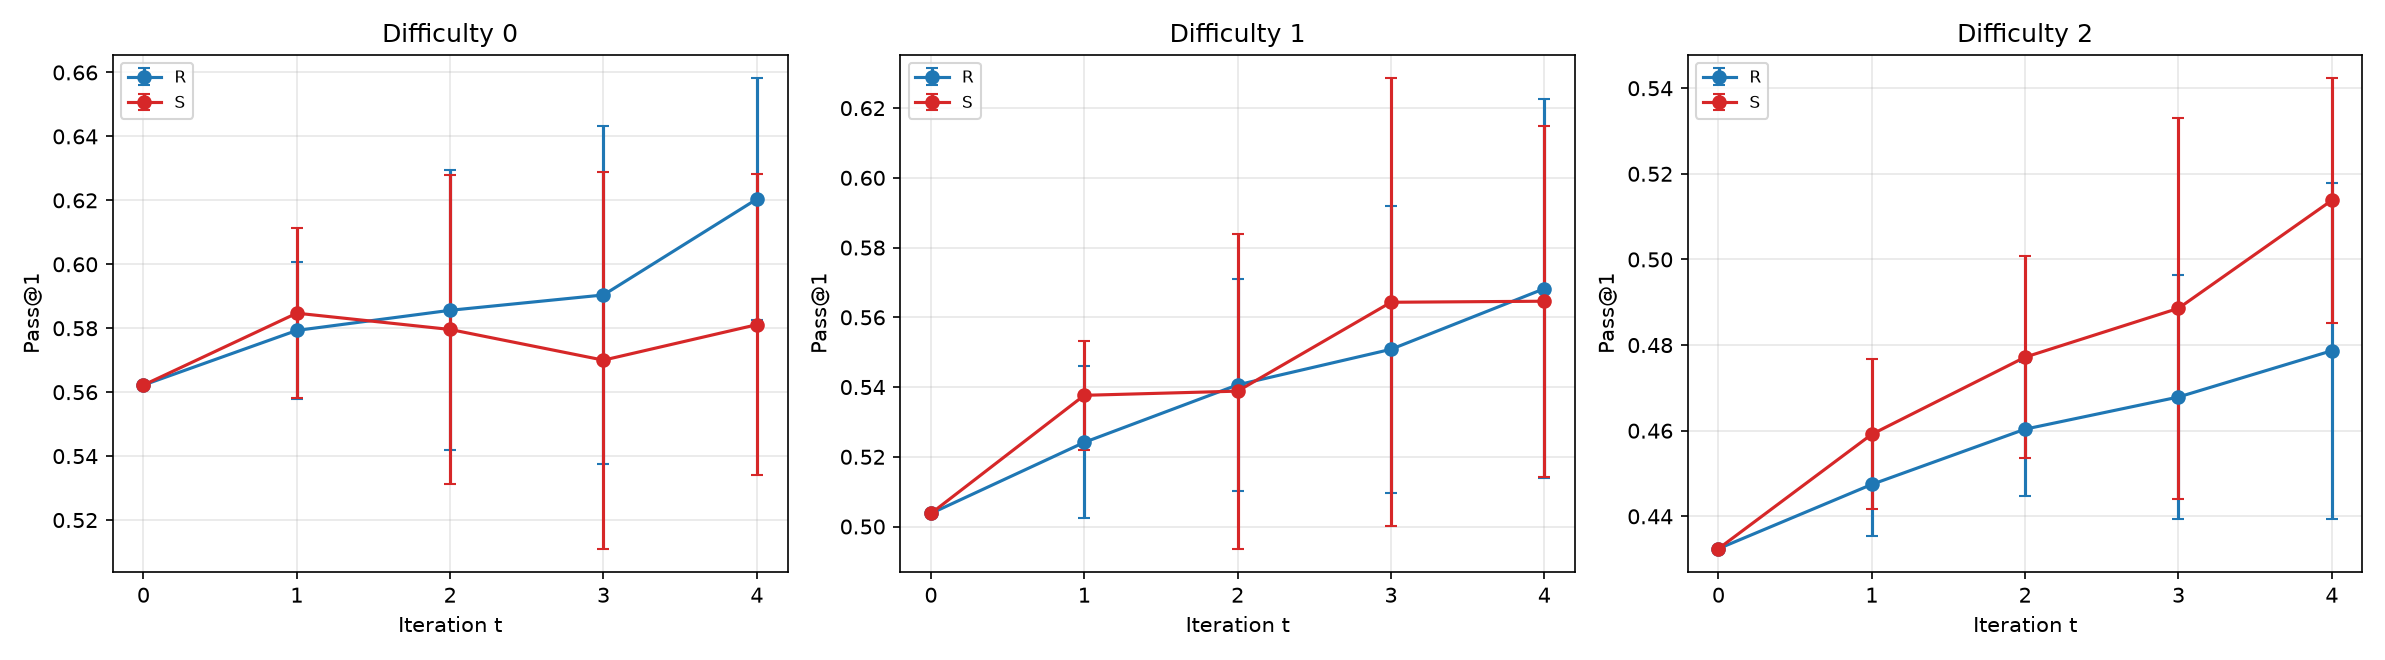
\includegraphics[width=0.90\linewidth]{figures/qwen_four_round_raw/unaudited_eval_id_by_difficulty.png}
\par\smallskip
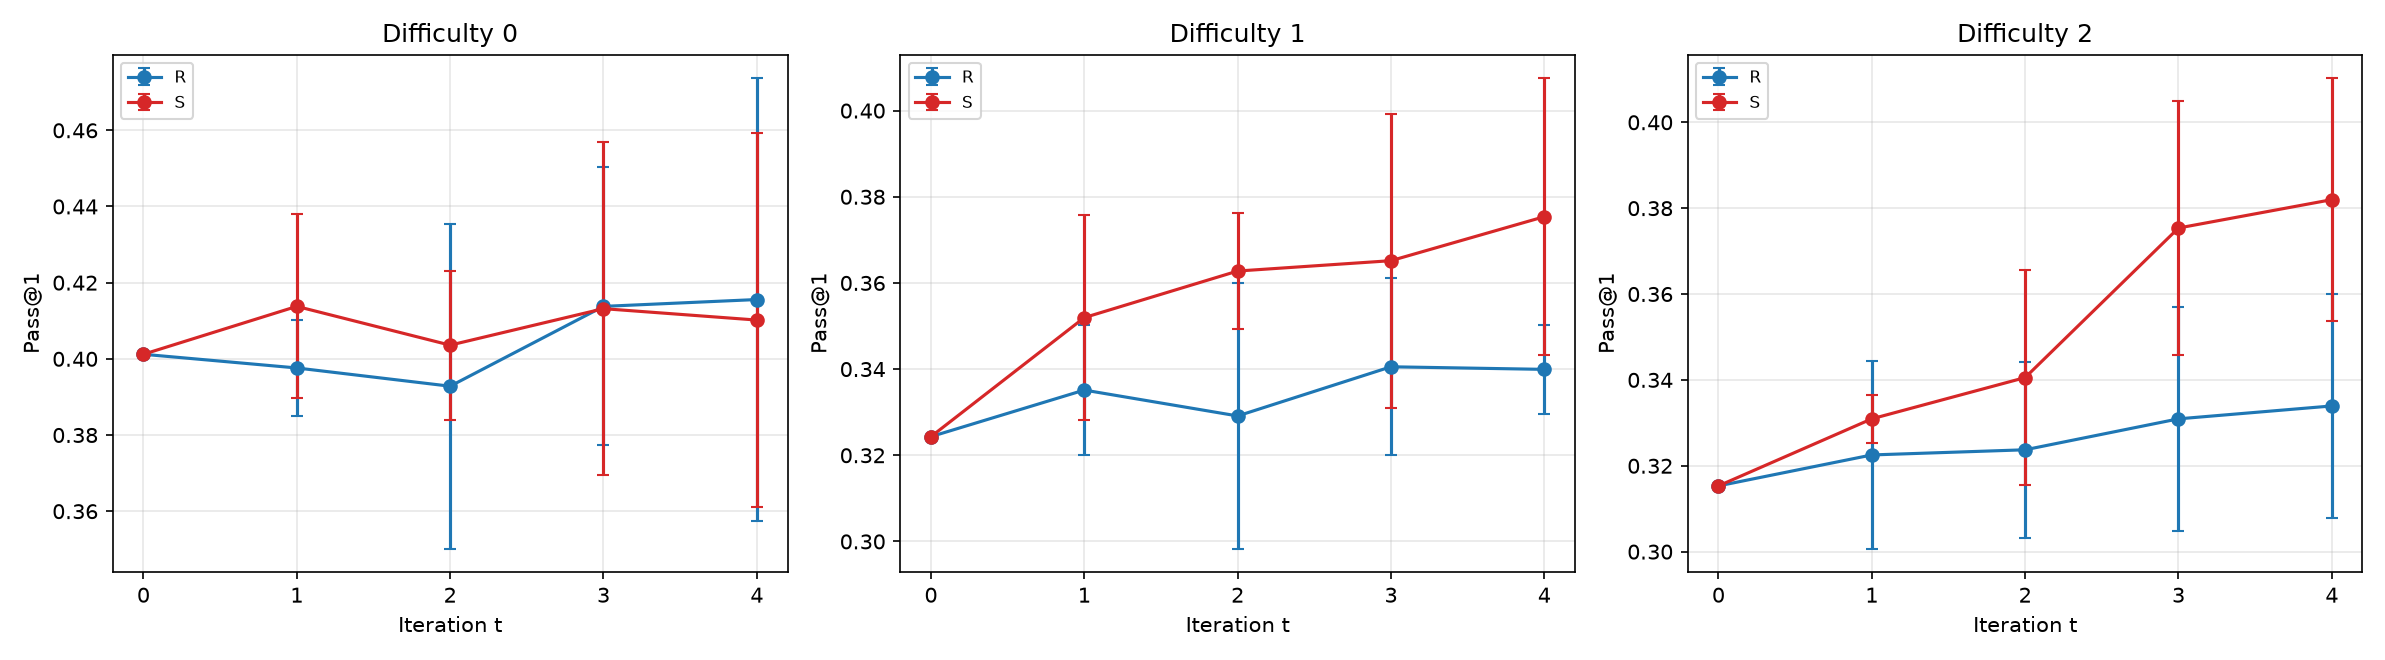
\includegraphics[width=0.90\linewidth]{figures/qwen_four_round_raw/unaudited_eval_ood_by_difficulty.png}
\caption{Original unaudited Qwen3-1.7B graph accuracy by generator
difficulty stratum, ID (top) and OOD (bottom), for rounds 0--4.
Strata 0--2 run from left to right and contain $667/667/666$ ID
and $334/333/333$ OOD questions. Error bars use the same five blocks
as Figure~\ref{fig:qwen-raw-unaudited}.}
\label{fig:qwen-raw-unaudited-difficulty}
\end{figure}

The strata are fixed features of the task generator, not an empirically
established ordering of model difficulty. Their separate vertical scales
are retained, so visual differences in slope do not by themselves
establish different learning rates. These descriptive trajectories
support no additional difficulty-specific significance claim.

\begin{figure}[H]
\centering
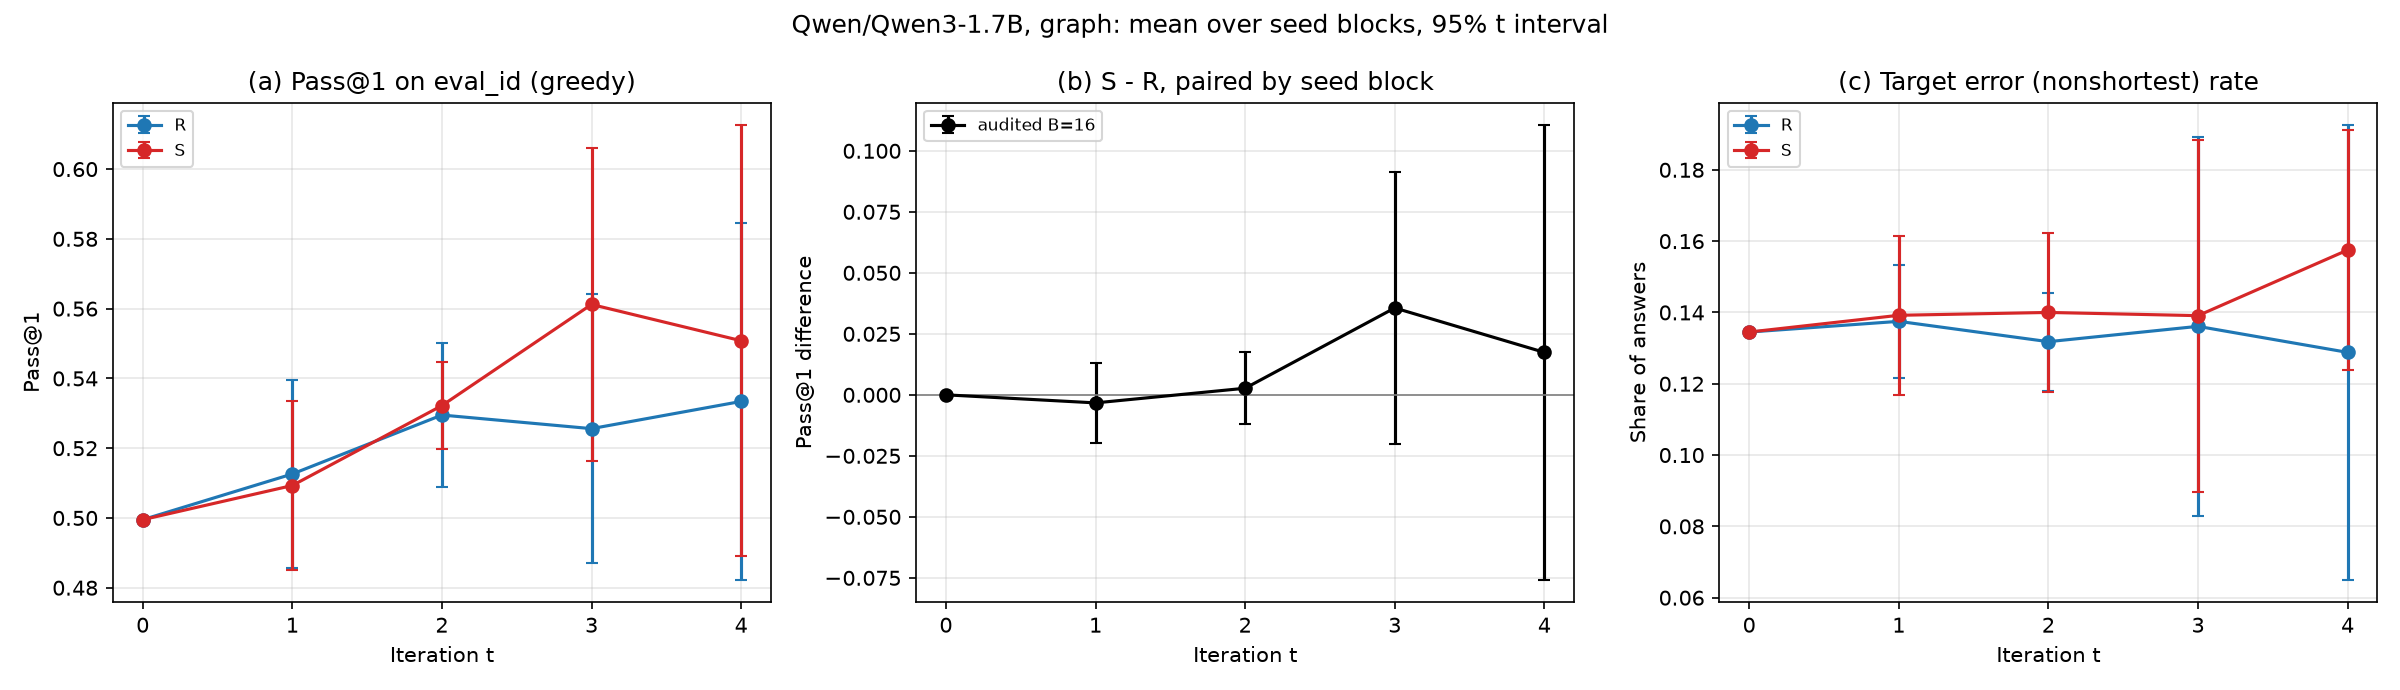
\includegraphics[width=0.90\linewidth]{figures/qwen_four_round_raw/audited_eval_id_pass1.png}
\par\smallskip
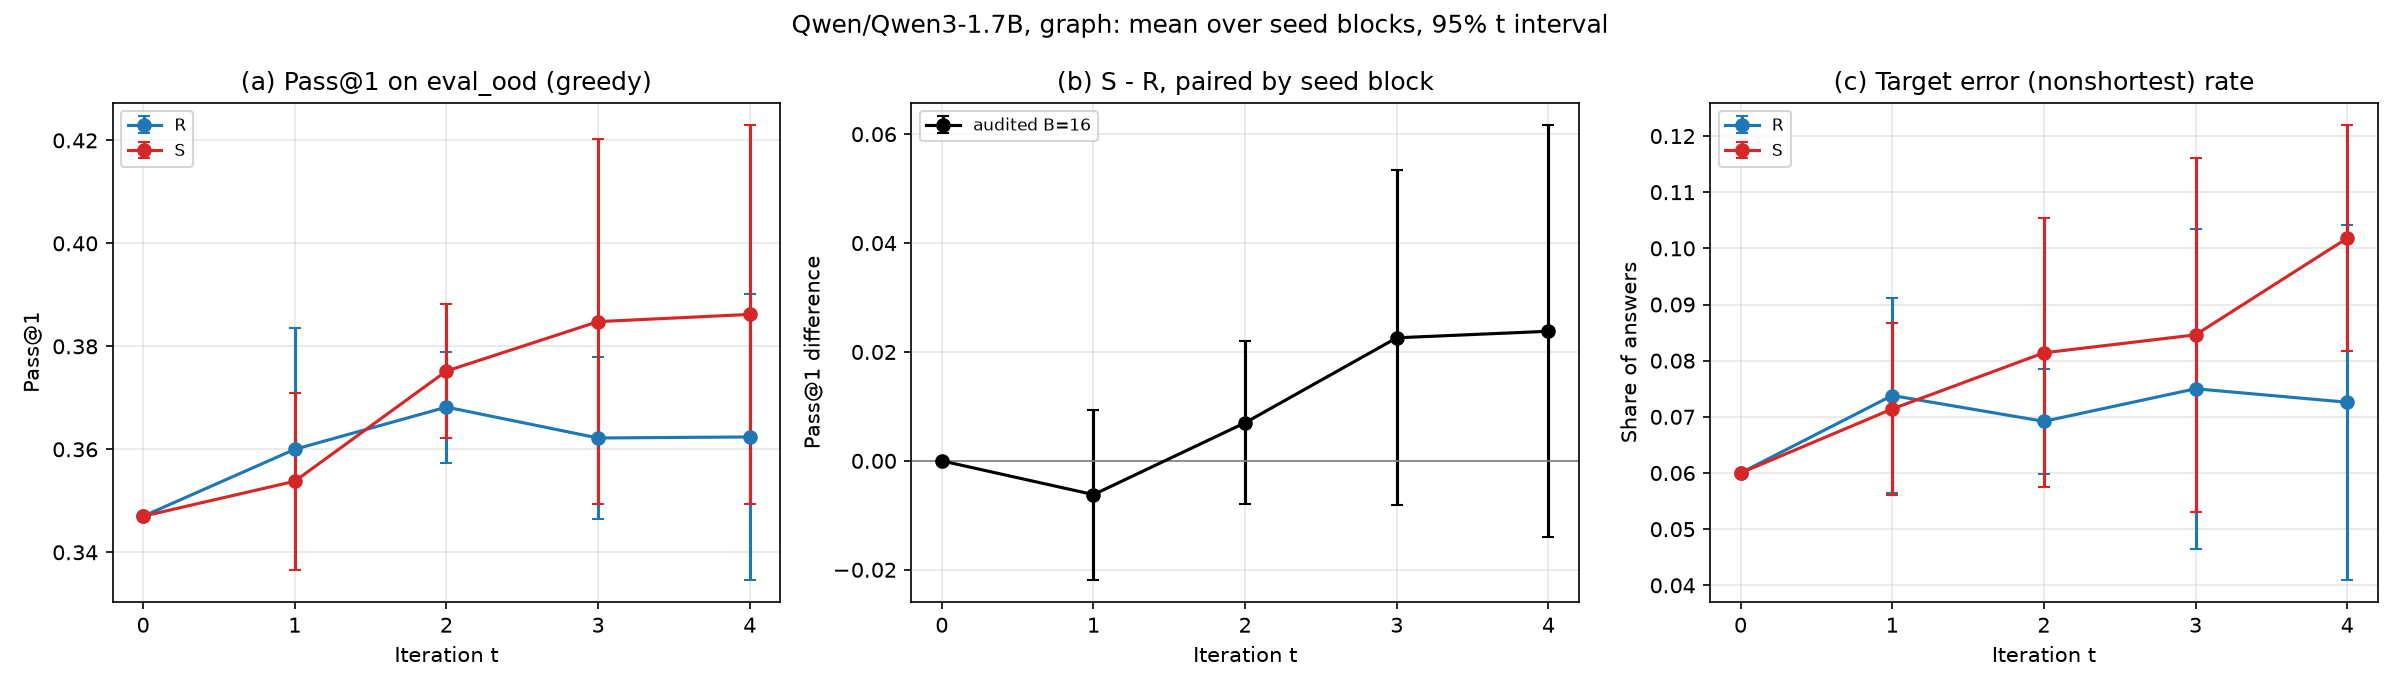
\includegraphics[width=0.90\linewidth]{figures/qwen_four_round_raw/audited_eval_ood_pass1.png}
\caption{Original adaptive-audit Qwen3-1.7B graph curves, ID (top)
and OOD (bottom), with $B_{\rm qry}=16$ correctness queries per
arm-round. The panels show greedy Pass@1, paired $S-R$ accuracy,
and nonshortest-error incidence. Each audited arm spends 64 queries
over four rounds.}
\label{fig:qwen-raw-audited}
\end{figure}

Under auditing, round-four $R/S$ accuracy is $0.533/0.551$ ID and
$0.362/0.386$ OOD. The paired contrasts are $0.017\pm0.093$ and
$0.024\pm0.038$, respectively. These contrasts
compare selection arms within the audited policy; they do not measure
the effect of adding an audit to an otherwise fixed training procedure.

\begin{figure}[H]
\centering
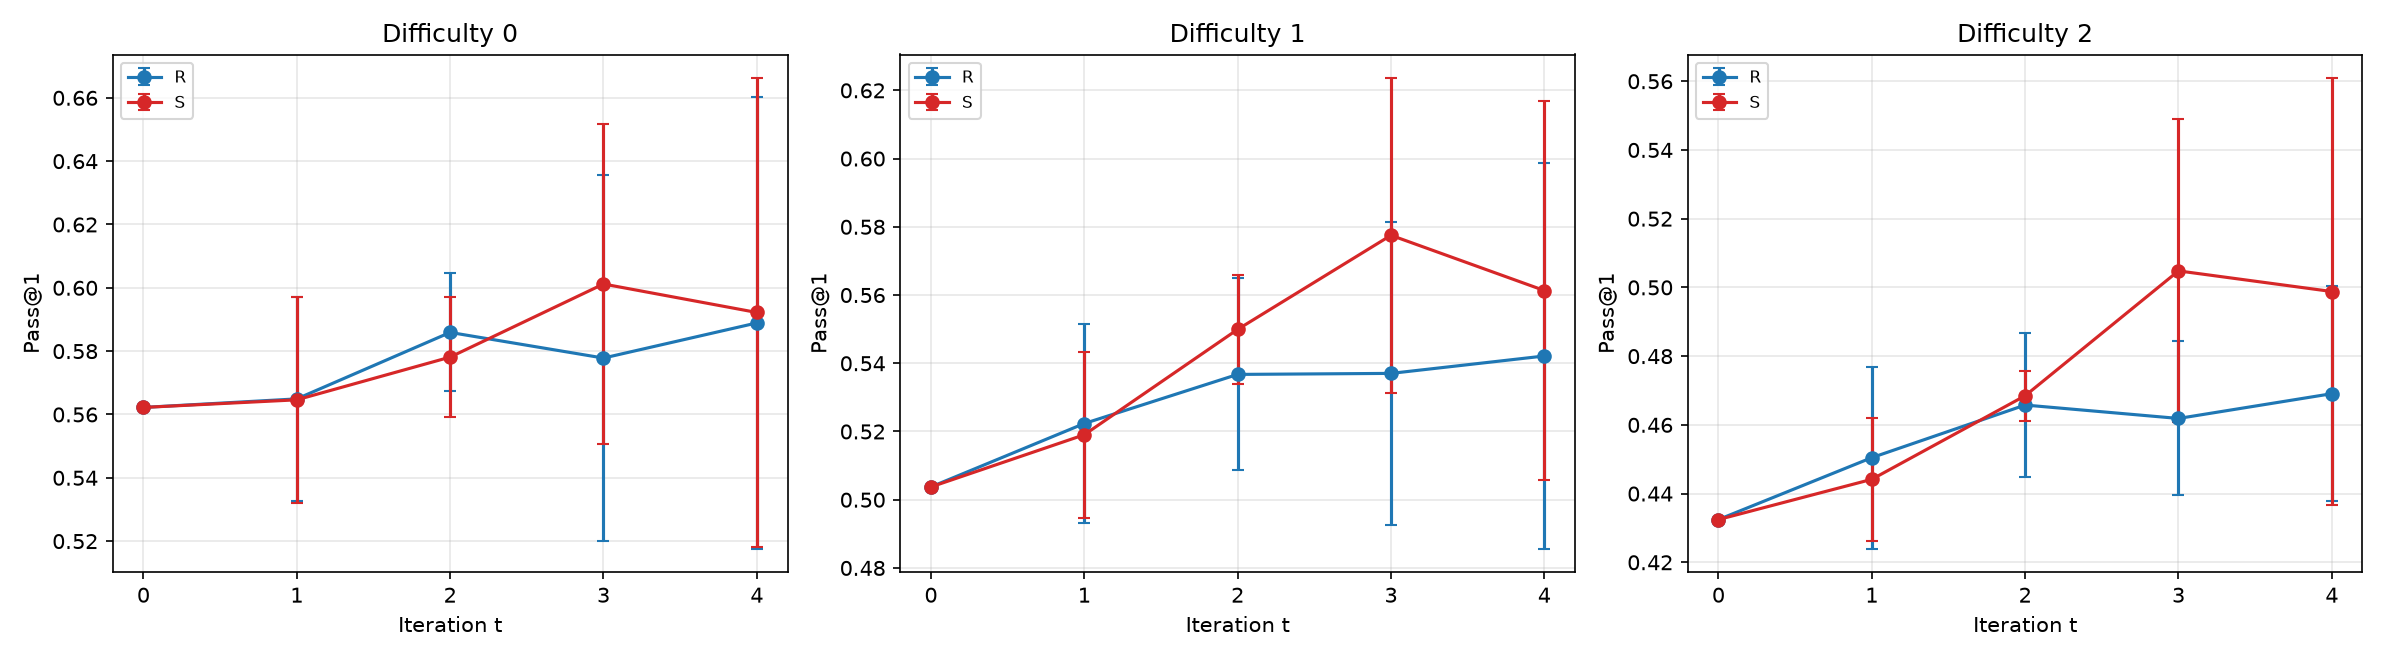
\includegraphics[width=0.90\linewidth]{figures/qwen_four_round_raw/audited_eval_id_by_difficulty.png}
\par\smallskip
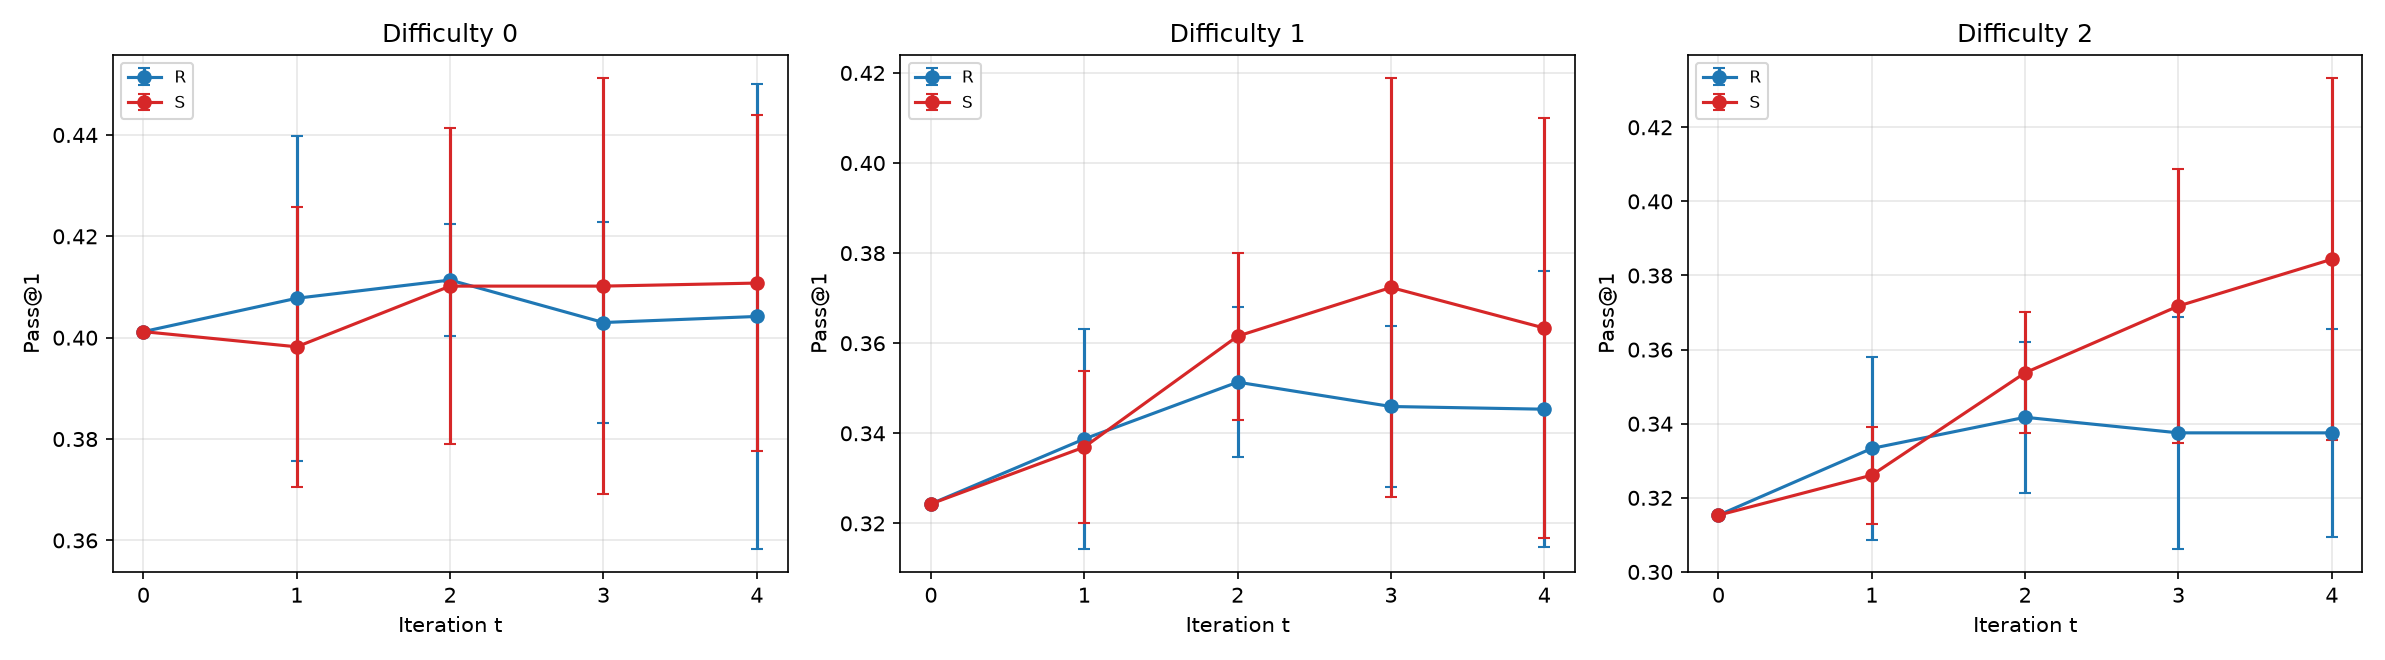
\includegraphics[width=0.90\linewidth]{figures/qwen_four_round_raw/audited_eval_ood_by_difficulty.png}
\caption{Original adaptive-audit Qwen3-1.7B graph accuracy by
generator stratum, ID (top) and OOD (bottom), for rounds 0--4.
The strata, fixed question sets, and pointwise block-$t$ intervals
follow Figure~\ref{fig:qwen-raw-unaudited-difficulty}.}
\label{fig:qwen-raw-audited-difficulty}
\end{figure}

The audited stratum curves supplement the aggregate results but do not
establish a stratum-specific audit benefit. They use the same fixed
questions as the unaudited curves, while retaining their original
separate vertical scales and pointwise uncertainty intervals.

\begin{figure}[H]
\centering
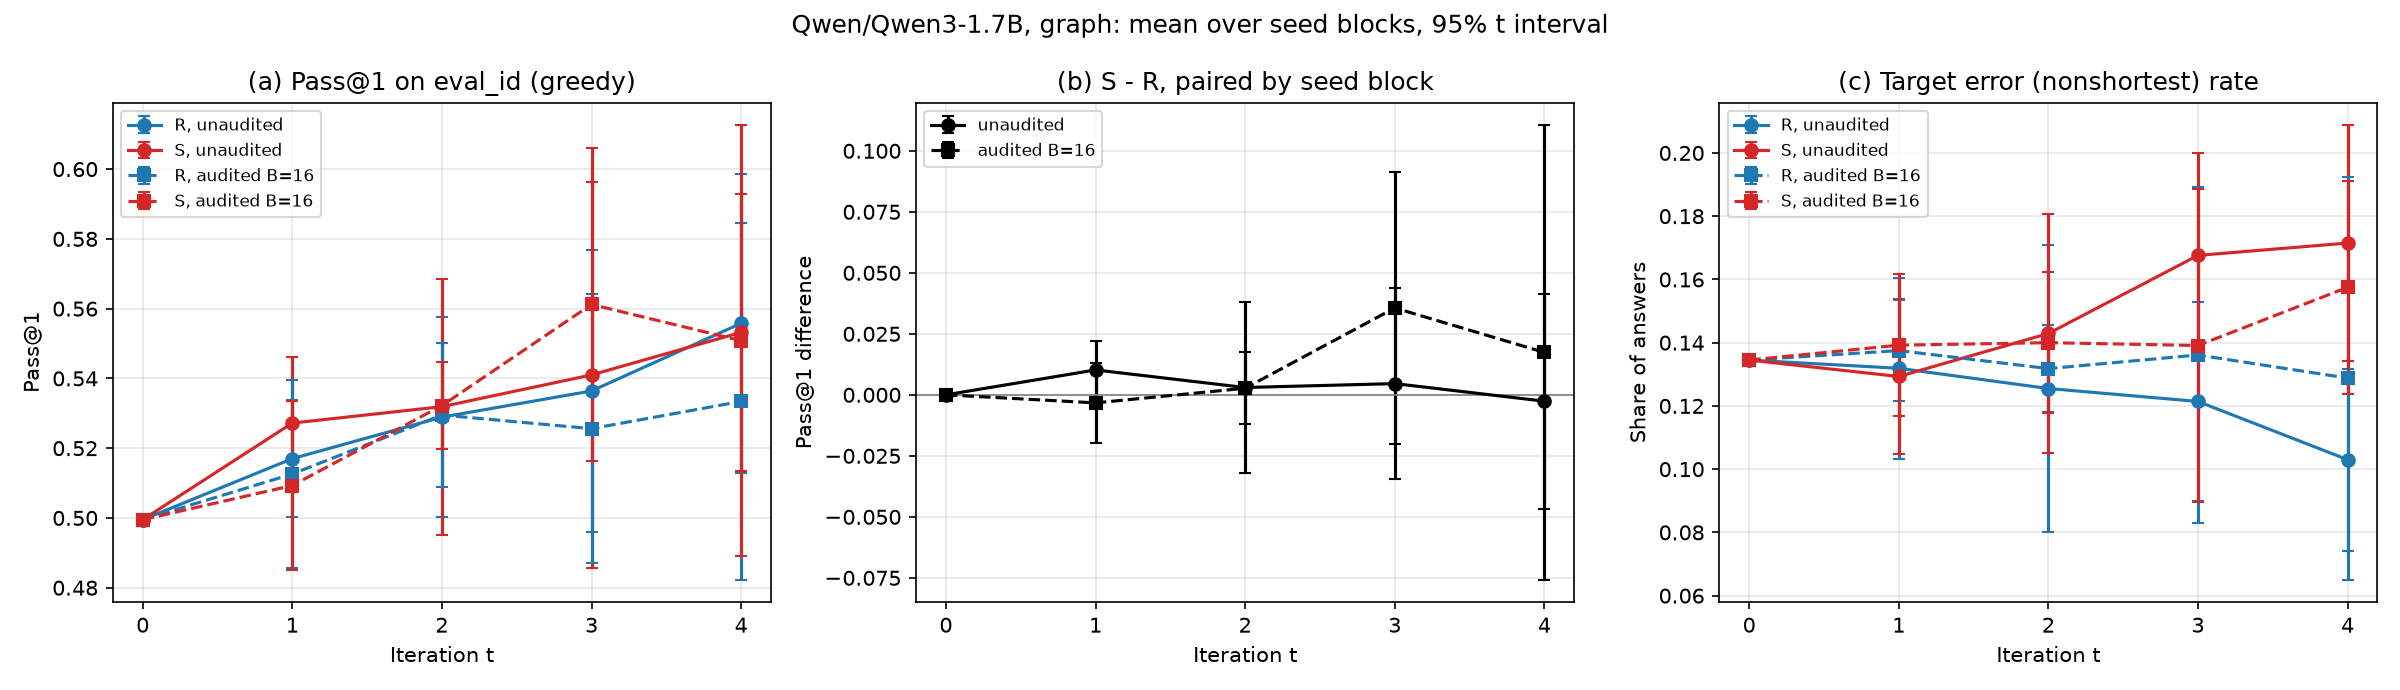
\includegraphics[width=0.90\linewidth]{figures/qwen_four_round_raw/comparison_eval_id_pass1.png}
\par\smallskip
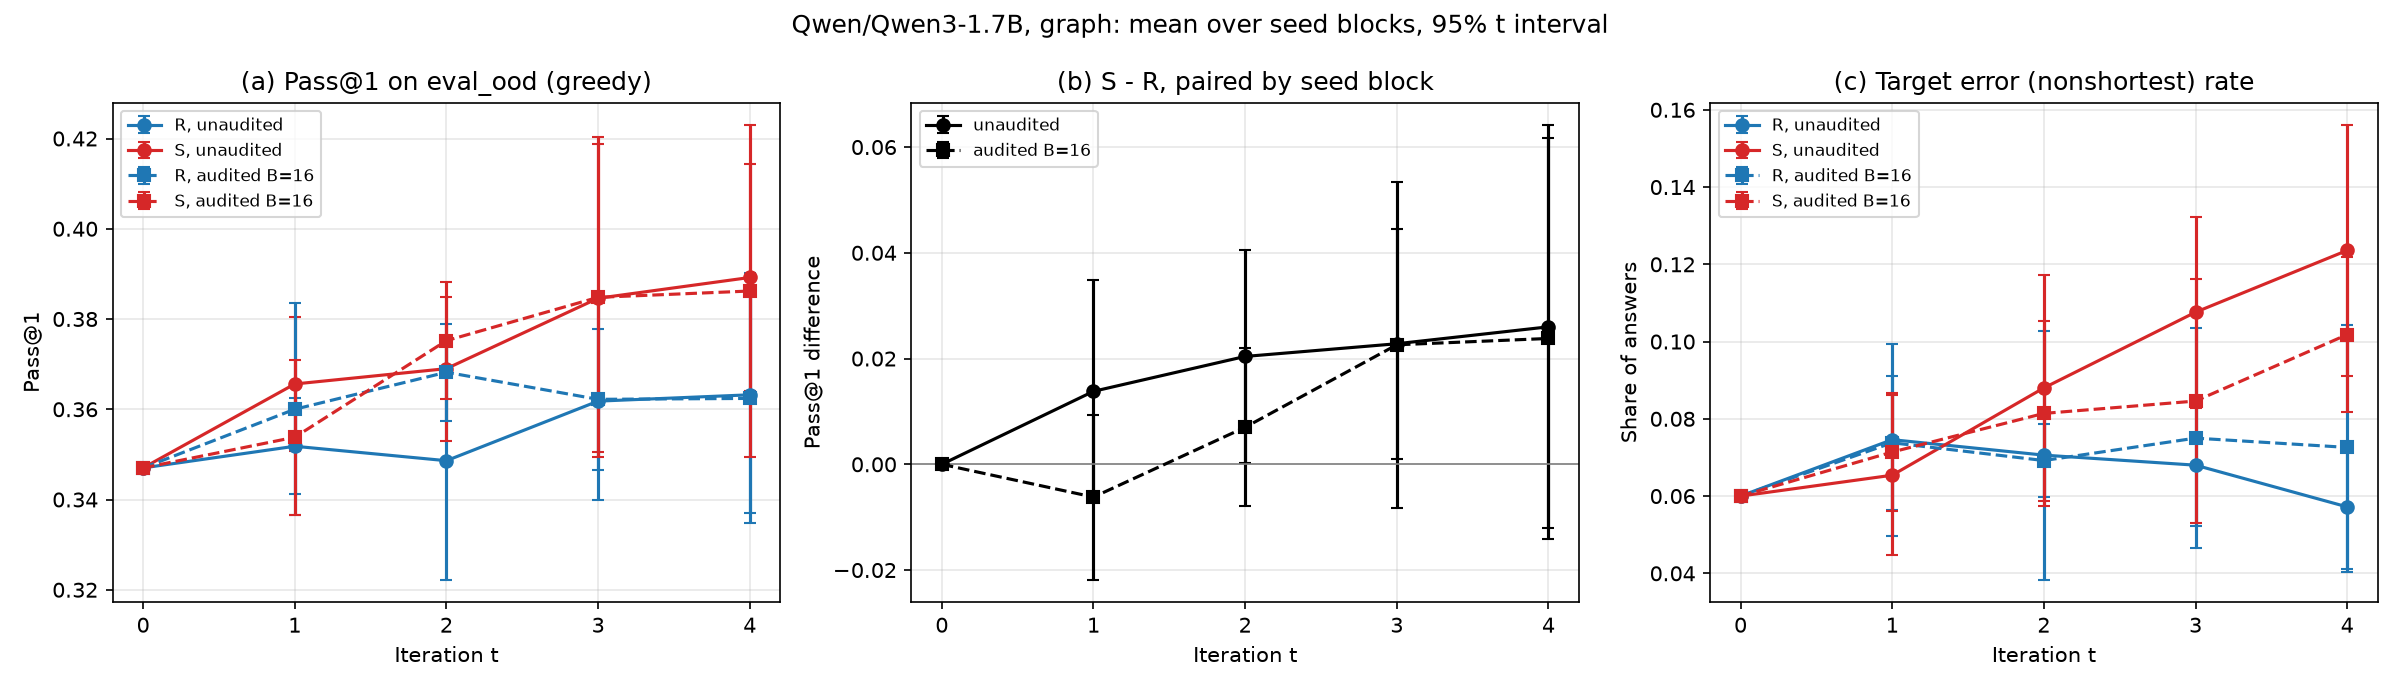
\includegraphics[width=0.90\linewidth]{figures/qwen_four_round_raw/comparison_eval_ood_pass1.png}
\caption{Original joint comparison of unaudited and adaptive-audit
Qwen3-1.7B graph trajectories, ID (top) and OOD (bottom), for
rounds 0--4. Each middle panel reports paired $S-R$ accuracy
separately within the two policies, not the effect of auditing.}
\label{fig:qwen-raw-comparison}
\end{figure}

Same-arm audited-minus-unaudited accuracy changes are negative in mean
(Table~\ref{tab:qwen-audit-change}).
The joint view therefore does not establish a uniform audit benefit;
it distinguishes within-policy arm differences from cross-policy changes.

\begin{figure}[H]
\centering
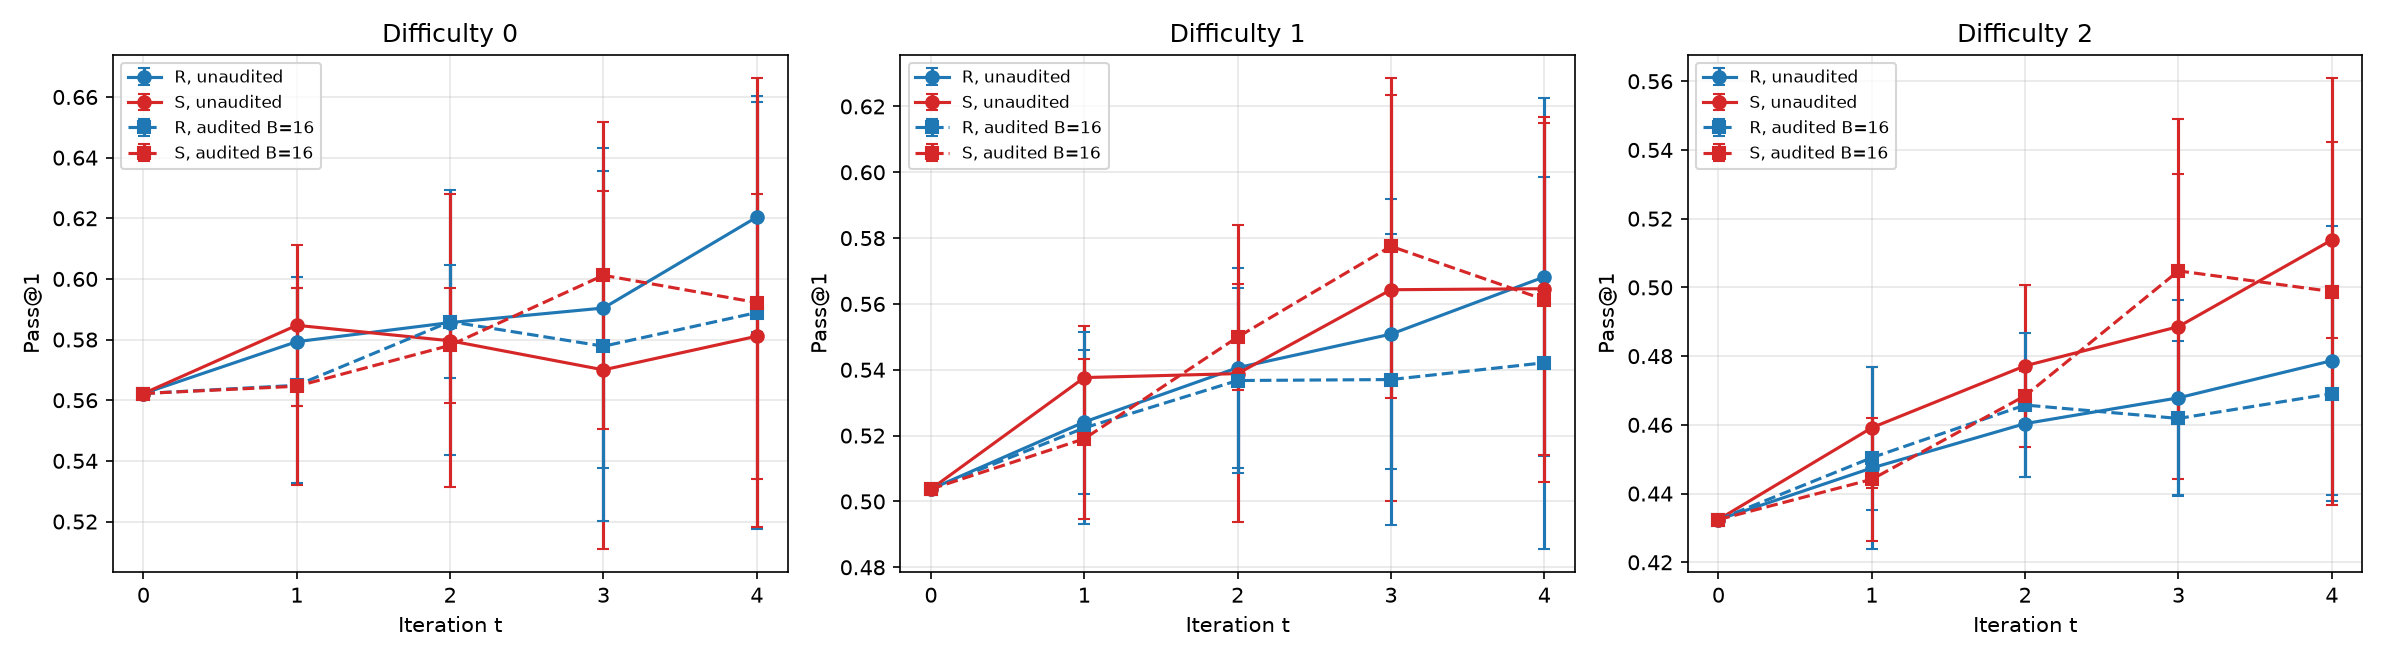
\includegraphics[width=0.90\linewidth]{figures/qwen_four_round_raw/comparison_eval_id_by_difficulty.png}
\par\smallskip
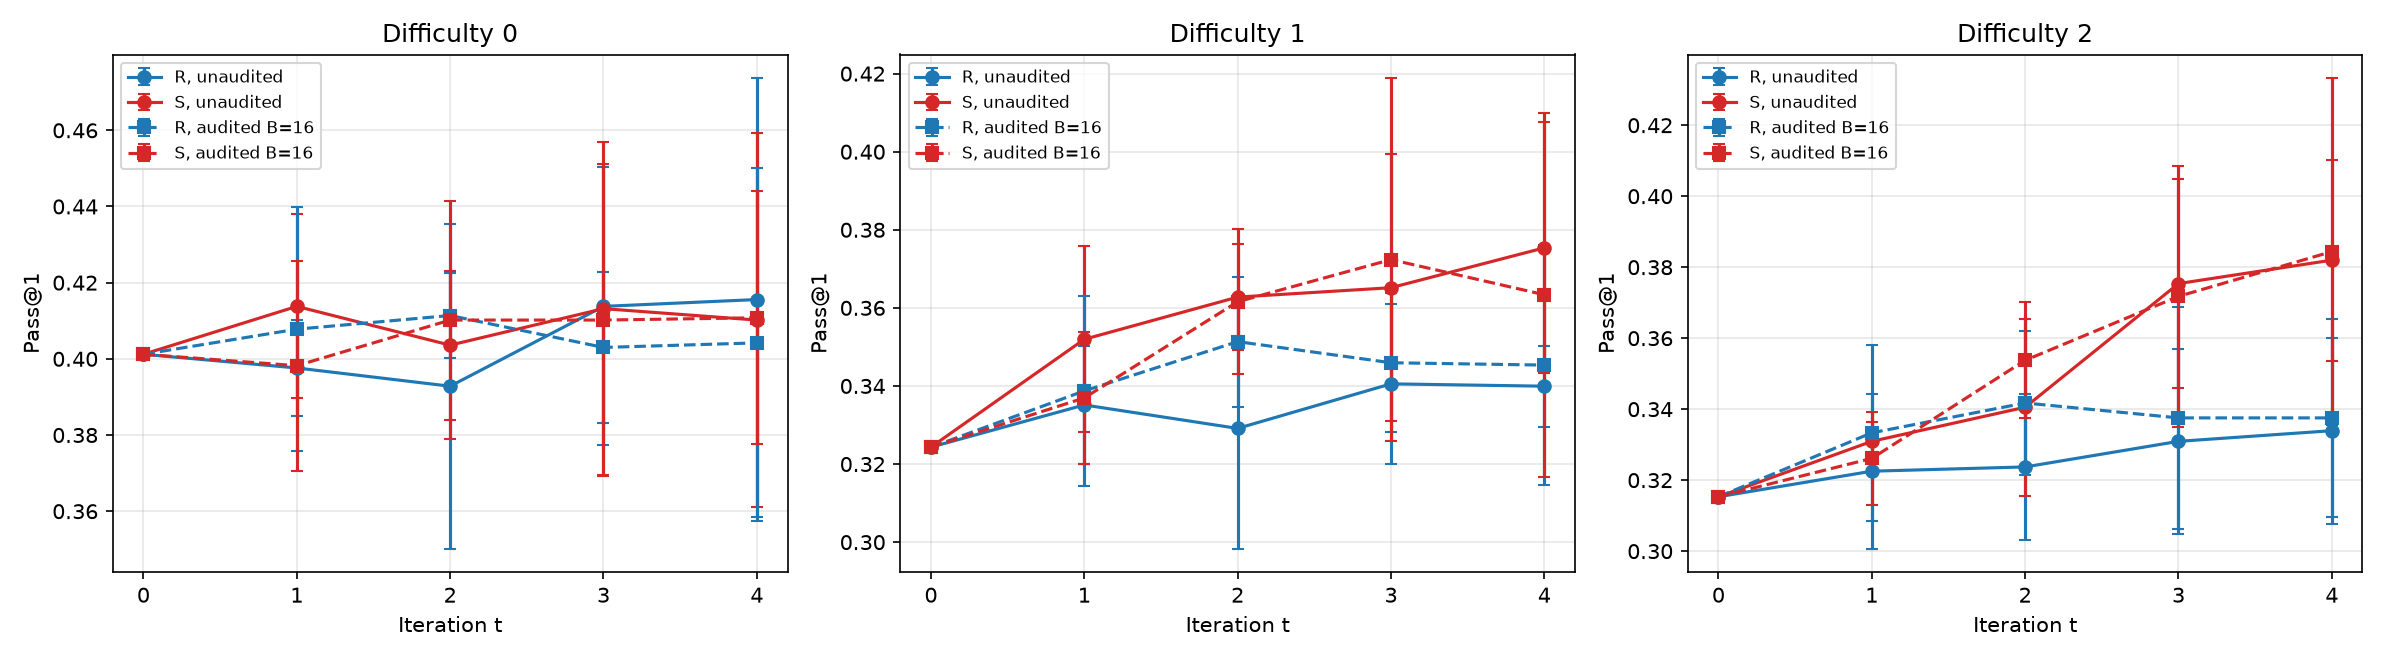
\includegraphics[width=0.90\linewidth]{figures/qwen_four_round_raw/comparison_eval_ood_by_difficulty.png}
\caption{Original joint Qwen3-1.7B graph accuracy curves by
generator stratum, ID (top) and OOD (bottom), for rounds 0--4.
Both policies and both arms use the same question stratum at
each checkpoint. Counts and interval conventions follow
Figure~\ref{fig:qwen-raw-unaudited-difficulty}.}
\label{fig:qwen-raw-comparison-difficulty}
\end{figure}

Both policies and both arms are evaluated on the same question stratum
at each checkpoint. Panel-specific vertical scales remain unchanged,
and the intervals are not adjusted for comparisons across strata,
rounds, or policies. The joint breakdown is consequently descriptive,
rather than a collection of confirmatory stratum-level tests.
\endgroup
